\section{Introduction}
\subsection{Course information}
\begin{frame}{Contacts}
    \textbf{Lecturer:} Václav B. Petrák  

    \textbf{Email:} vaclav.petrak@fbmi.cvut.cz  

    \textbf{Phone/WhatsApp:} +420 725 878 390

    \vspace{1em}
    \textbf{Consultations:} 
    \begin{itemize}
        \item In person: after individual request. Please mail me or text me.
        \item In person: on Friday 2\textsuperscript{nd} on May 2025 for project-related problems
        \item By email any time
    \end{itemize}

\end{frame}

\begin{frame}{Absence Policy}
\begin{itemize}
    \item \textbf{Advance Notice Required:} All absences must be excused in advance whenever possible.

    \item \textbf{Communication Procedure:}  Contact me  as soon as possible by email with date of absence a reason for the absence.

    \item \textbf{Responsibility for Missed Work:} You will be are responsible for making up missed assignments, by following the content of course materials.  
\end{itemize}
 

\end{frame}

\begin{frame}{Lectures}
\Large
\begin{itemize}
    \item We will have 5 topics in modeling and simulation, each for one day.
    \item The last lecture will be focused on presentation of your work. 
\end{itemize}
\end{frame}

\begin{frame}{Classification}
\begin{center}
    \Large
    There is no exam.
    
    \vspace{1em}
    %\pause
    Your grade will be based on your independent work. There are three outputs used for grading.
    %\pause

    \vspace{1em}
    \color{primary}
    \textbf{1. Journal Club Presentation\\\small30\% of the final grade }
    
    %\pause
    \vspace{1em}
    \color{primary}
    \textbf{2. Capstone Project Presentation\\\small40\% of the final grade} 

    \vspace{1em}
    \color{primary}
    \textbf{3. Code Review Discussion\\\small30\% of the final grade}
    
    
\end{center}
\end{frame}

\begin{frame}{Journal Club is a discussion of research papers.}
   A journal club is a group who meet to critically evaluate  articles in the academic literature. Journal clubs:
     \begin{itemize}
        \item Encourages critical thinking.
        \item Helps in understanding the studied concepts and methods.
        \item Helps keep up with the latest research.
        \item Improves communication and presentation skills.
        \item Presentation simulates experience of a scientist
    \end{itemize}
\vspace{1em}
\textbf{The main purpose in this course is to explore how methods we learned are applied in current research}
    
\end{frame}

\begin{frame}{Your Task for Journal Club}
    \begin{itemize}
        \item You will read a research paper related to the topic of your capstone project.
        \item Your task is to read the paper and prepare a 15-minute presentation, followed by a 5-minute discussion, to explain the paper.
       \item The presentation dates will be arranged individually. 
    \end{itemize}
\end{frame}

\begin{frame}{The Journal Club presentation will cover:}
    \begin{itemize}
    \small
        \item \textbf{Introduction:} Provide a High-level Overview on the background of the research topic and the main objectives of the paper.
        \item \textbf{Methods:} Give overview of the methodology used in the paper.
        \item \textbf{Results:} Highlight the key results and conclusions of the paper.
        \item \textbf{Discussion:} Discuss the practical implications of the research and its applications in real-world situations. Discuss any limitations of the paper.
        \item \textbf{Conclusions:} Summarize the main contributions and overall findings of \textbf{the paper}. Reiterate its key takeaways and their broader implications.
        \item \textbf{Q\&A:} Answer questions from the audience (lecturer)
    \end{itemize}
\end{frame}

\begin{frame}[t]{Grading Criteria for Journal Club Presentation}
\only<1-2>{
 \textbf{Presentation Design and Delivery (50\%)}
    \begin{itemize}
     \footnotesize
        \item \textbf{Design:} The presentation is well-organized and easy to follow
        \item \textbf{Timing:} The presenter adhered to the 15-minute presentation format.
        \item \textbf{Delivery:} Clear and confident speech with appropriate pacing.
         \item \textbf{Questions}  Convincing response to questions.
    \end{itemize}
    }
\vspace{1em}
\only<2>{   
 \textbf{Content of the presentation (50\%)}
    \begin{itemize}
     \footnotesize
       \item \textbf{Introduction:} The introduction provides a high-level overview of the topic: explains the research motivation and the research question.
       \item \textbf{Methods:} Explains the experimental approach used by the authors. Unfamiliar methods are explained without going into excessive detail.
       \item \textbf{Results:} The key results from the paper are explained.
        \item \textbf{Critical evaluation:} For example critique of methods, ideas for improvement, significance of the results.
    \end{itemize}
}
\end{frame}

\begin{frame}{Capstone project is your independent project}
\begin{columns}
    \begin{column}{0.55\textwidth}
        \begin{itemize}
            \item You will work on independent project that builds on and further extends course content.  
            \item Output of your work will be a presentation and a code. 
            \item The presentation dates will be arranged individually. 
        \end{itemize}
    \end{column}
    %\pause
    \begin{column}{0.45\textwidth}
    \footnotesize
    \begin{center}
        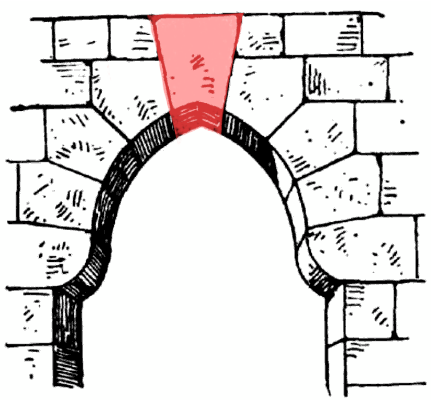
\includegraphics[scale = 0.75]{lesson_1/images/capstone.png} 
        \end{center}
    \vspace{1em}
       \textit{ A  \textbf{capstone} (or keystone) is the wedge-shaped stone at the apex of an arch. \textbf{It is the final piece placed during construction and locks all the stones into position}, allowing the arch to bear weigh.}
 
    \end{column}
\end{columns}
\end{frame}

\begin{frame}{The Capstone Project presentation will cover:}
    \begin{itemize}
        \small
        \item \textbf{Introduction:} Provide a High-level Overview on the background of the research topic and the main objectives of \textbf{your project}.
        \item \textbf{Methods:} Give overview of the methodology used in \textbf{your project}.
        \item \textbf{Results:} Highlight the key results and conclusions of \textbf{your project}.
        \item \textbf{Discussion:} Discuss the practical implications of \textbf{your project's findings} and their applications in real-world situations. Discuss any limitations of \textbf{your project}.
        \item \textbf{Conclusions:} Summarize the main contributions and overall findings of \textbf{your project}. Reiterate its key takeaways and their broader implications.
        \item \textbf{Q\&A:} Answer questions from the audience (lecturer) 
    \end{itemize}
\end{frame}

\begin{frame}[t]{Grading Criteria for Capstone Project}
\only<1-2>{
 \textbf{Presentation Design and Delivery (50\%)}
    \begin{itemize}
     \footnotesize
        \item \textbf{Design:} The presentation is well-organized and easy to follow
        \item \textbf{Plots:} Clear graphical presentation of simulation results that address project objectives and show model behavior.
        \item \textbf{Timing:} The presenter adhered to the 15-minute presentation format.
        \item \textbf{Delivery:} Clear and confident speech with appropriate pacing.
         \item \textbf{Questions}  Convincing response to questions.
    \end{itemize}
    }
\vspace{1em} % This space will appear on slide step 2, between the two main sections

  \only<2>{
 \textbf{Model Implementation (50\%)}
    \begin{itemize}
         \footnotesize
        \item \textbf{Correctness:} Correct function of fundamental models. 
        \item \textbf{Understanding:} Demonstrated understanding of core concepts.
        \item \textbf{Extension beyond core:} Successful and meaningful implementation of additional features (if the task specifies them).
        \item \textbf{Discussion:} Insightful discussion on how parameters/initial conditions affect outcomes. Identification and explanation of  behaviors.
    \end{itemize}

  } % End of \only for Project Development and Critical Evaluation

\end{frame}

\begin{frame}[t]{During Code Review we will discuss your code.}
Code Review assesses the \textbf{your understanding}, quality, design, and documentation of the Capstone Project code.
\vspace{1em}

\begin{itemize}
\small
    \item \textbf{Primary Focus:} The review concentrates on code for the Capstone Project. 
    \item \textbf{Interactive Session:} Review involves an interactive code walk-through you will explain your code's functionality and design choices.
    \item \textbf{Demonstrating Ownership:} This is an opportunity for you to demonstrate your good understanding of the project, justify the decisions made during development, and articulate the purpose of different code segments.
    \item \textbf{Goal:} The ultimate goal is to ensure the correctness of your project, while demonstrating your grasp of the implemented concepts.
\end{itemize}
\end{frame}

\begin{frame}[t]{Grading Criteria for Code Review}
\only<1-2>{
 \textbf{Readability and Maintainability (20\%)}
    \begin{itemize}
        \footnotesize
        \item Clean, well-formatted, and easy to follow code.
        \item Consistent naming conventions and style.
        \item Logical organization: functions that brake code into manageable components in neceessary.
        \item Sufficient and meaningful comments for complex/non-obvious code.
    \end{itemize}
    \vspace{0.5em}
    }
\only<2>{
\textbf{Code understanding (80\%)}
    \begin{itemize}
    \footnotesize
        \item Ability to explain how any part of the code works.
        \item Ability to clearly articulate design decisions and justify coding choices made during development.
        \item Ability to suggest improvements, extensions or alternatives.
    \end{itemize}

}
\end{frame}

\begin{frame}{Avoid using AI to solve entire exercises}
    \begin{itemize}
        \item Consider a math problem: 
        \begin{itemize}
            \item \textit{Given that two trains are traveling on parallel tracks in opposite directions with speeds of 56 km/h and 52 km/h, respectively, and lengths of 136 m and 242 m, respectively, after what duration will they cross each other?}
        \end{itemize}
        %\pause
        \item The primary goal is \textbf{not} to find the answer but to practice your reasoning and calculation skills.
           %\pause
        \item Similarly,  the aim of modeling and simulation exercises is to learn and practice new skills.
           %\pause
        \item Avoid using generative AI like ChatGPT or Gemini to solve the \textbf{entire problem} for you.      
        \begin{itemize}
            \item It spoils learning process for you
            \item It may disrupt pacing of the lesson. 
        \end{itemize}
    \end{itemize}
\end{frame}

\begin{frame}{Using AI During Lessons} % More direct title
\Large 
During lessons, you may use AI to:

\begin{itemize}
    \item Ask clarifying questions. 
    \item Debug your code: after you've made your own attempts. 
    \item Get ideas for further work. 
\end{itemize}

\vspace{0.5cm}  % Increased spacing

\begin{center}
\textbf{Let's discuss what is a fair use of generative AI in the capstone project} 
\end{center}
\end{frame}

\subsection{Introduction to Modeling}
\begin{frame}[t]{Model is a representation of a \textbf{system}}
\small
 \begin{columns}
 \begin{column}{0.65\textwidth}
     \begin{itemize}
    \item    A model is a representation of a \textbf{system} that enables us investigate its properties and \textbf{predict} future outcomes.
    \begin{itemize}
           \item    A \textbf{system} is  a set of components  that interact with each other within a boundary to function as a whole: Solar system, rabbit and fox populations, a microscope
           
       \end{itemize}
    \item In modeling we aim to identify components, relationships and behavior to predict system dynamics.
       \only<2->{
        \item Modeling always requires simplification (abstraction)
       }
      \only<3>{
         \item  \textbf{A mathematical model uses mathematical equations to describe a system.}}
    \end{itemize}
 \end{column}

 \begin{column}{0.35\textwidth}
 \color{primary}

\only<1>{
\begin{center}
   
\includegraphics[scale = 0.15]{lesson_1/images/dummy.png}  
\end{center}}

 \only<2>{
 Example of a model: 
SIR (susceptible, infectious, and recovered) model for dynamics of infectious diseases
\vspace{1em}

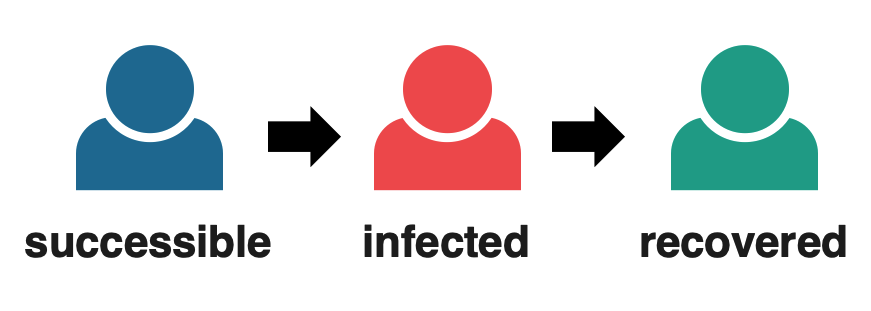
\includegraphics[scale = 0.12]{lesson_1/images/sir.png}
 }
  \only<3>{
 SIR  model equations:
\begin{align*}
    \frac{dS}{dt} &= -\beta S I \\
    \\
    \frac{dI}{dt} &= \beta S I - \gamma I \\
    \\
    \frac{dR}{dt} &= \gamma I
  \end{align*}
 }
 \end{column}
 \end{columns} 
\end{frame}

{
\setbeamercolor{background canvas}{bg=black}
\setbeamercolor{normal text}{fg=white}
\begin{frame}
\begin{center}
\large
    \color{white} % This ensures that the text is white
    All models are approximations. Assumptions, whether implied or clearly stated, are never exactly true.
    %\pause
    
    \vspace{1em}
    \textbf{All models are wrong, but some models are useful.} 

    %\pause
    
    \vspace{1em}
    So the question you need to ask is not \textit{Is the model true?} 
    
        %\pause
    \vspace{1em}   
    It never is.
        %\pause

    \vspace{1em}
    But \textit{Is the model good enough for this particular application?}
  \vfill % This ensures vertical space is added before your text at the bottom
\hfill --- George E. P. Box % This will align "George E. P. Box" to the right
\end{center}


\end{frame}
}
